\documentclass{article}

\usepackage{graphicx}
\usepackage{url}

\begin{document}

\title{CSE6801 Distributed Computing Systems\\
(Bully Leader Election Algorithm)}
\author{Name: Md. Khaledur Rahman, St.Id: 0413052039\\ Name: Mostafizur Rahman, St.Id: 0413052072\\Name: Subir Saha, St.Id:0413052048}
\maketitle

\section*{Introduction:}
The bully algorithm is a method in distributed computing system for dynamically electing a coordinator by process ID number. The process with the highest process ID number is selected as the coordinator. The bully algorithm assumes that the system is synchronous. Each processes knows which processor has the higher identifier number and communicates with that. There is another assumption that the connection is reliable. However, prior information about other process id's must be known. In the following sections, we have discussed about our implementation of bully algorithm.

\section*{Implementation:}

In this assignment, we have implemented the bully selection algorithm. We have used Python v2.7.6 for our implementation. Our algorithm is given as follows:

\begin{itemize}
\item Process P broadcasts an election message `Election' to all other processes with higher process IDs, expecting an `Answer' response from them if they are alive.
\item If P hears from no process with a higher process ID than it, it wins the election and broadcasts victory.
\item If P hears from a process with a higher ID, P waits a certain amount of time for any process with a higher ID to broadcast itself as the leader. If it does not receive this message in time, it re-broadcasts the election message.
\item If P gets an election message `Election' from another process with a lower ID it sends an `Answer' message back and starts new elections.
\end{itemize}

When a node P (process) gets `Answer' message from all of its neighbouring processes, then it announces itself as leader. All the nodes then set P as leader if none of them have any objection. Basically, in our implementation, node with highest ID has the maximum probability of being selected as leader. 

We have also implemented bully algorithm when network gets partitioned somehow. In that case, we assumed that only odd nodes can communicate with odd ids and even ids can communicate with even ids. So, here will be two leaders, one from odd nodes and another from even nodes.

\section*{Discussion:}

We have shown a graph (see fig.\ref{fig:image}) counting number of nodes (processes) vs. number of election messages passed among different processes for the case when network does not get partitioned. To conduct experiment, we have used 10, 20, 30, 40 and 50 nodes. It shows that number of messages passed increase linearly with increased number of nodes (processes).
\begin{figure}
    \centering
    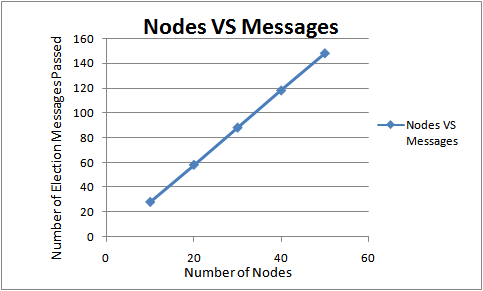
\includegraphics[width=0.8\textwidth]{bully.png}
    \caption{Number of Nodes (Processes) vs. Number of Election messages passed}
    \label{fig:image}
\end{figure}

\begin{thebibliography}{1}

\bibitem{wiki} \url{http://en.wikipedia.org/wiki/Bully_algorithm}

\bibitem{gm} Garcia-Molina, H., \emph{Elections in Distributed Computing System}, IEEE Transaction  Computers, Vol.C-1,pp.48-59,Jan.1982.

\bibitem{st} Stoller, S. D., \emph{Leader Election in Distributed Systems with Crash Failures}, Indiana University, Bloomington, IN 47405, USA.

\bibitem {tanen} Tanenbaum, A.S., and Steen M.V.,  \emph{Distributed Systems Principles and Paradigms},  Prentice-Hall International, Inc, 2002. Sample Chapter. 

\end{thebibliography}

\end{document}